\section{Bayesian Analysis}

In this section, we discuss the Bayesian analysis of the normal mean.
Assuming our data $X | \mu \sim N(\mu, \sigma^2)$, where $\sigma$ is known, we have:

\[ f(x | \mu) = \frac{1}{\sigma \sqrt{2\pi}} \exp\left(-\frac{(x - \mu)^2}{2\sigma^2}\right) \]

The likelihood function, given the sample $\bar{x} = (x_1, x_2, \dots, x_n)$, can be calculated as:

\begin{align*}
  L(\mu | \bar{x}) &= \prod_{i = 1}^{n} f(x_i | \mu) \\
  &= \prod_{i = 1}^{n} \frac{1}{\sigma \sqrt{2\pi}} \exp\left(-\frac{(x_i - \mu)^2}{2\sigma^2}\right) \\
  &\propto \exp\left(-\frac{\sum_{i = 1}^{n} (x_i - \mu)^2}{2\sigma^2}\right) \\
  &\propto \exp\left(-\frac{\sum_{i = 1}^{n} (\mu^2 - 2x_i ~ \mu + x_i^2)}{2\sigma^2}\right) \\
  &\propto \exp\left(-\frac{n \mu^2 - 2\sum_{i = 1}^{n} x_i ~ \mu + \sum_{i = 1}^{n} x_i^2}{2\sigma^2}\right) \\
  &\propto \exp\left(-\frac{n \mu^2 - 2\sum_{i = 1}^{n} x_i ~ \mu}{2\sigma^2}\right) \\
  &\propto \exp\left(-\frac{n}{2\sigma^2} \left(\mu^2 - 2\sum_{i = 1}^{n} x_i / n ~ \mu\right)\right) \\
  &\propto \exp\left(-\frac{n}{2\sigma^2} \left(\mu - \sum_{i = 1}^{n} x_i / n\right)^2\right) \\
\end{align*}

Supose $\mu \sim N(u, v)$ is the prior distribution of $\mu$, then:

\begin{align*}
  f(\mu) &= \frac{1}{\sqrt{2\pi v}} \exp\left(-\frac{(\mu - u)^2}{2v}\right) \\
  &\propto \exp\left(-\frac{\mu^2 - 2u \mu + u^2}{2v}\right) \\
  &\propto \exp\left(-\frac{\mu^2 - 2u \mu}{2v}\right)
\end{align*}

The posterior distribution will be:

\begin{align*}
  f(\mu | \bar{x}) &\propto f(\mu) \cdot L(\mu | \bar{x}) \\
  &\propto \exp\left(-\frac{\mu^2 - 2u \mu}{2v}\right) \cdot \exp\left(-\frac{n \mu^2 - 2\sum_{i = 1}^{n} x_i ~ \mu}{2\sigma^2}\right) \\
  &\propto \exp\left(-\frac{\mu^2 - 2u \mu}{2v} - \frac{n \mu^2 - 2\sum_{i = 1}^{n} x_i ~ \mu}{2\sigma^2}\right) \\
  &\propto \exp\left(-\frac{1}{2v \sigma^2} \left((n v + \sigma^2) \mu^2 - 2(u \sigma^2 + v \sum_{i = 1}^{n} x_i ~ \mu)\right)\right) \\
  &\propto \exp\left(-\frac{n v + \sigma^2}{2v \sigma^2} \left(\mu - \frac{u \sigma^2 + v \sum_{i = 1}^{n} x_i}{n v + \sigma^2}\right)^2\right) \\
  &\propto \exp\left(-\frac{1}{2v'} (\mu - u')^2\right)
\end{align*}

\noindent where $u' = \left(u \sigma^2 + v \sum_{i = 1}^{n} x_i\right) / (n v + \sigma^2)$ and $v' = v \sigma^2/(n v + \sigma^2)$.
The kernel of the posterior distribution shows that $\mu | \bar{x} \sim N(u', v')$.


\subsection{Bayesian Analysis with Different Sample Sizes}

We can clearly see that the posterior mean is a weighted average of the prior mean and the "likelihood mean":

\begin{align*}
  u' &= \frac{1}{n v + \sigma^2} \left(u \sigma^2 + v \sum_{i = 1}^{n} x_i\right) \\
  &= \frac{1}{v + \sigma^2 / n} \left(u \sigma^2 / n + v \sum_{i = 1}^{n} x_i / n\right) \\
  &= \frac{\sigma^2 / n}{v + \sigma^2 / n} \cdot u + \frac{v}{v + \sigma^2 / n} \cdot \sum_{i = 1}^{n} x_i / n \\
  &= w_n \cdot u + (1 - w_n) \cdot \sum_{i = 1}^{n} x_i / n
\end{align*}

where $w_n = \frac{\sigma^2 / n}{v + \sigma^2 / n}$.
We can also see that $\lim_{n \to \infty} w_n = 0$, implying that as $n \to \infty$ (as data size increases), the posterior mean is shifted towards the likelihood mean.

Also, the posterior precision, defined as $p' = 1 / v'$, is sum of the prior precision ($p = 1 / v$) and likelihood precision ($p_L = n / \sigma^2$) as shown below:

\begin{align*}
  p' &= \frac{1}{v'} = \frac{n v + \sigma^2}{v \sigma^2} \\
  &= \frac{n}{\sigma^2} + \frac{1}{v} \\
  &= p_L + p
\end{align*}

\noindent Note that $p_L \to \infty$ and $p' \to \infty$ as $n \to \infty$.

Refer to \autoref{fig:post} to visualize these effects.

\begin{figure}[!ht]
  \centering
  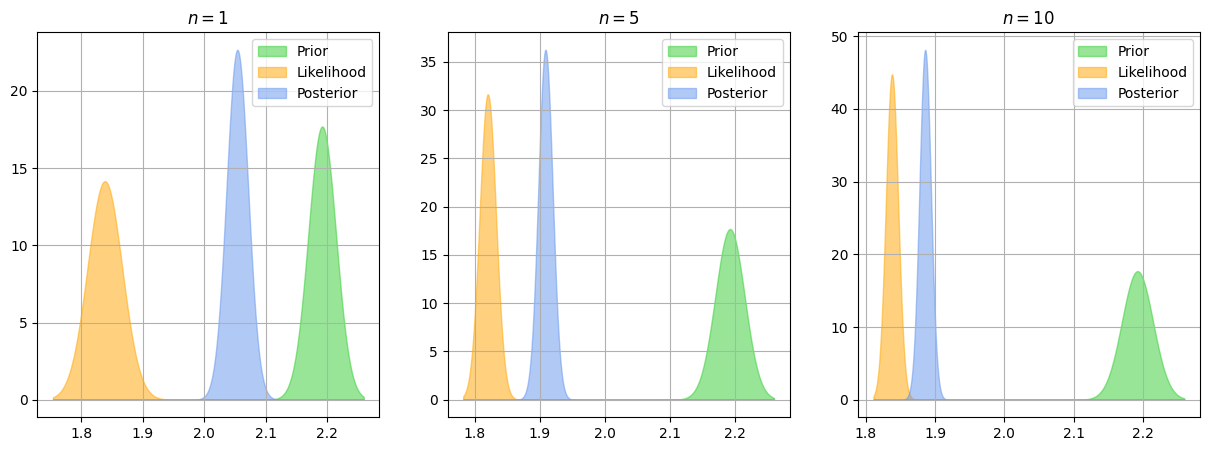
\includegraphics[width=\textwidth]{images/posterior.png}
  \caption{Effects of sample size on the posterior distribution}
  \label{fig:post}
\end{figure}
